\section{LSM9DS1}
Der benyttes en IC (LSM9DS1), som både indeholder magnometer, gyroskop og accelerometer. Det er muligt at indstille accelerometeret til $\pm$1, 4, 8 eller 16 g. Gyroskopet kan måle $\pm$245, 500 eller 2000 grader per sekund, og magnometeret kan måle $\pm$4, 8, 12 eller 16 G.\citep{Jimb02016} \newline
LSM9DS1 har ni frihedsgrader, hvormed det måler i x-, y- og z-aksen for både magnometeret, gyroskopet og accelerometeret, hvilket kan ses på \figref{vores_IC}. Akserne for gyroskopet og accelerometeret internt følger højrehåndsreglen, mens magnometerets x- og y-akse er flippet.\citep{Jimb02016}

\begin{figure}[H]
	\centering
	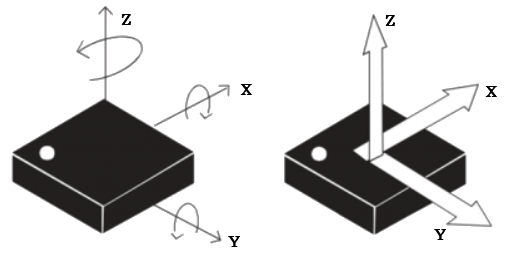
\includegraphics[scale=0.6]{figures/cDesign/LSM9DS1.png}
	\caption{På figuren ses akserne fra IC'en LSM9DS1, hvor magnometerets (til venstre) akse i realiteten er flippet i forhold til gyroskopet (i midten) og accelerometeret (til højre).\citep{Jimb02016}}
	\label{fig:sensor_placering}
\end{figure}

LSM9DS1 er valgt, da den både indeholder et gyroskop og et accelerometer, som der er mulige at benytte enkeltvis eller samlet. Da gyroskopet bruger 4mA og accelerometeret bruger 600$\text muA$, er det væsentligt at kunne sætte gyroskopet i sleepmode, når dette ikke benyttes. 